\chapter{Approach}

This capstone report aims to develop a method to calibrate the extrinsic parameters of a multiple partially overlapping RGB-D camera system. Each camera in the system already has the intrinsic parameters (from the manufacturer), so this report just focuses on extrinsically calibrating. The approach consists of two main parts: the first section proposes the double-sided ArUco board as the calibration target and estimates the relative pose between the board and each camera in the system, and the second part mentions the application of the General Graph Optimisation in our method.

\clearpage
\section{Camera model}
% The expected rate of events is $\lambda$. 

It is essential to obtain a good established mathematical modelling that correctly defines the operating of a typical camera to handle the calibration. In this method, the pinhole camera model is used to describe a 3D point $P(X, Y, Z)$ in the global frame to a 2D image plane position $p(u, v)$ via a projection matrix $M$.
\[
s
\begin{bmatrix}
    u \\
    v \\
    1
\end{bmatrix}
=M
\begin{bmatrix}
    X \\
    Y \\
    Z \\
    1
\end{bmatrix}
\]

The projection matrix $M$ combines the intrinsic parameters $K$ and the extrinsic parameters $[R, T]$ for a camera in a specific setup.
\[
M=K[R T]
\]

To determine the relative pose between cameras in the system (also known as the extrinsic parameters), firstly, we have to estimate the transformation from the calibration target (in this case is the ArUco board) to each camera. To optimise the calibration result, this work is performed continuously throughout the calibration process. All the transformation (translation and rotation) between the cameras to the ArUco board during the calibration process are recorded for the Pose Graph Optimisation.

The Perspective-n-Point (PnP) pose computation problem is reviewed to detect the ArUco board pose respected to the camera frame. This method estimates the relative transform (translation and rotation) between a calibrated camera (with all the intrinsic parameters) and a 3D target, minimising the re-projection error from the 2D-3D point.
\clearpage

\begin{figure}[ht]
\centering
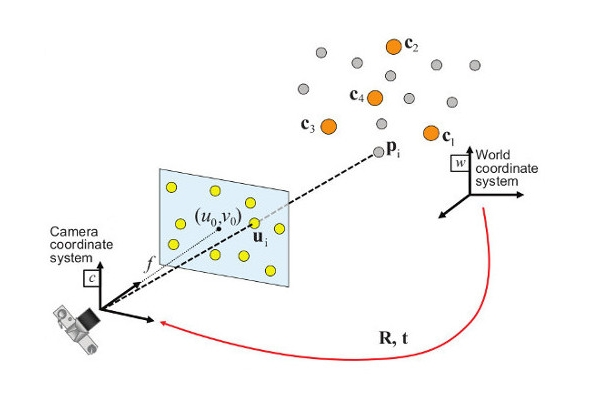
\includegraphics[width=1\textwidth]{Images/Perspective-n-Point (PnP) pose problem.jpg}
\caption{Perspective-n-Point (PnP) pose problem}
\end{figure}

Theoretically, we have a set of 3D points within a global frame of reference and their respective 2D image projections. Assuming the camera has been intrinsically calibrated already and the camera matrix is defined, we are able to determine the relative pose (position and orientation) between the camera itself and the global frame. This follows the projecting model in perspective for the cameras:
\[
p_{I}=K[RT]p_{W}
\]
In which:

$p_{W}=[X_{W}, Y_{W}, Z_{W}, 1]$: the global point coordinates in homogeneous form.

$p_{I}=[u,v,1]$: the respective image point coordinates in homogeneous form.

$
K=
\begin{bmatrix}
    f_{x} &  0      & c_{x} \\
    0     &  f_{y}  & c_{y} \\
    0     &  0      & 1
\end{bmatrix}
$
a matrix includes the intrinsic parameters, also known as camera matrix. $f_{x}$, $f_{y}$ is the focal length and $c_{x}$, $c_{y}$ is the principal point.

$R, T$: 3D rotation and translation matrix (extrinsic parameters).

This results in the formula equation of the model:
\[
\begin{bmatrix}
    u \\
    v \\
    1
\end{bmatrix}
=
\begin{bmatrix}
    f_{x} &  0      & c_{x} \\
    0     &  f_{y}  & c_{y} \\
    0     &  0      & 1
\end{bmatrix}
\begin{bmatrix}
    r_{11} &  r_{12} & r_{13} & t_{x} \\
    r_{21} &  r_{22} & r_{23} & t_{y} \\
    r_{31} &  r_{32} & r_{33} & t_{z} \\
    0      &  0      & 0      & 1
\end{bmatrix}
\begin{bmatrix}
    X_{W} \\
    Y_{W} \\
    Z_{W} \\
    1
\end{bmatrix}
\]

Therefore, the relative pose combines the 3D translation and the 3D rotation, which transforms a 3D object in the global frame into the camera frame:
\[
\begin{bmatrix}
    X_{C} \\
    Y_{C} \\
    Z_{C} \\
    1
\end{bmatrix}
=
\begin{bmatrix}
    r_{11} &  r_{12} & r_{13} & t_{x} \\
    r_{21} &  r_{22} & r_{23} & t_{y} \\
    r_{31} &  r_{32} & r_{33} & t_{z} \\
    0      &  0      & 0      & 1
\end{bmatrix}
\begin{bmatrix}
    X_{W} \\
    Y_{W} \\
    Z_{W} \\
    1
\end{bmatrix}
\]

\clearpage
\section{Calibration target configuration: double-sided ArUco board}
We propose a double-sided planar board configuration with a set of ArUco markers as the calibration target. The board's thickness is carefully measured to the nearest 0.1 millimetres. The ArUco markers are printed on paper and mounted on both sides of the board, following the given order. These markers are the same size with given side lengths. In addition, to simplify the detection process, the $[x, y, z]$ coordinates of 4 corners of the ArUco markers are determined, which is respected to the board's origin frame. Finally, the origin coordinate frame of the double-sided board is identified in the lower-left corner of the front side of the board.
\vspace{5mm}

\begin{figure}[ht]
\centering
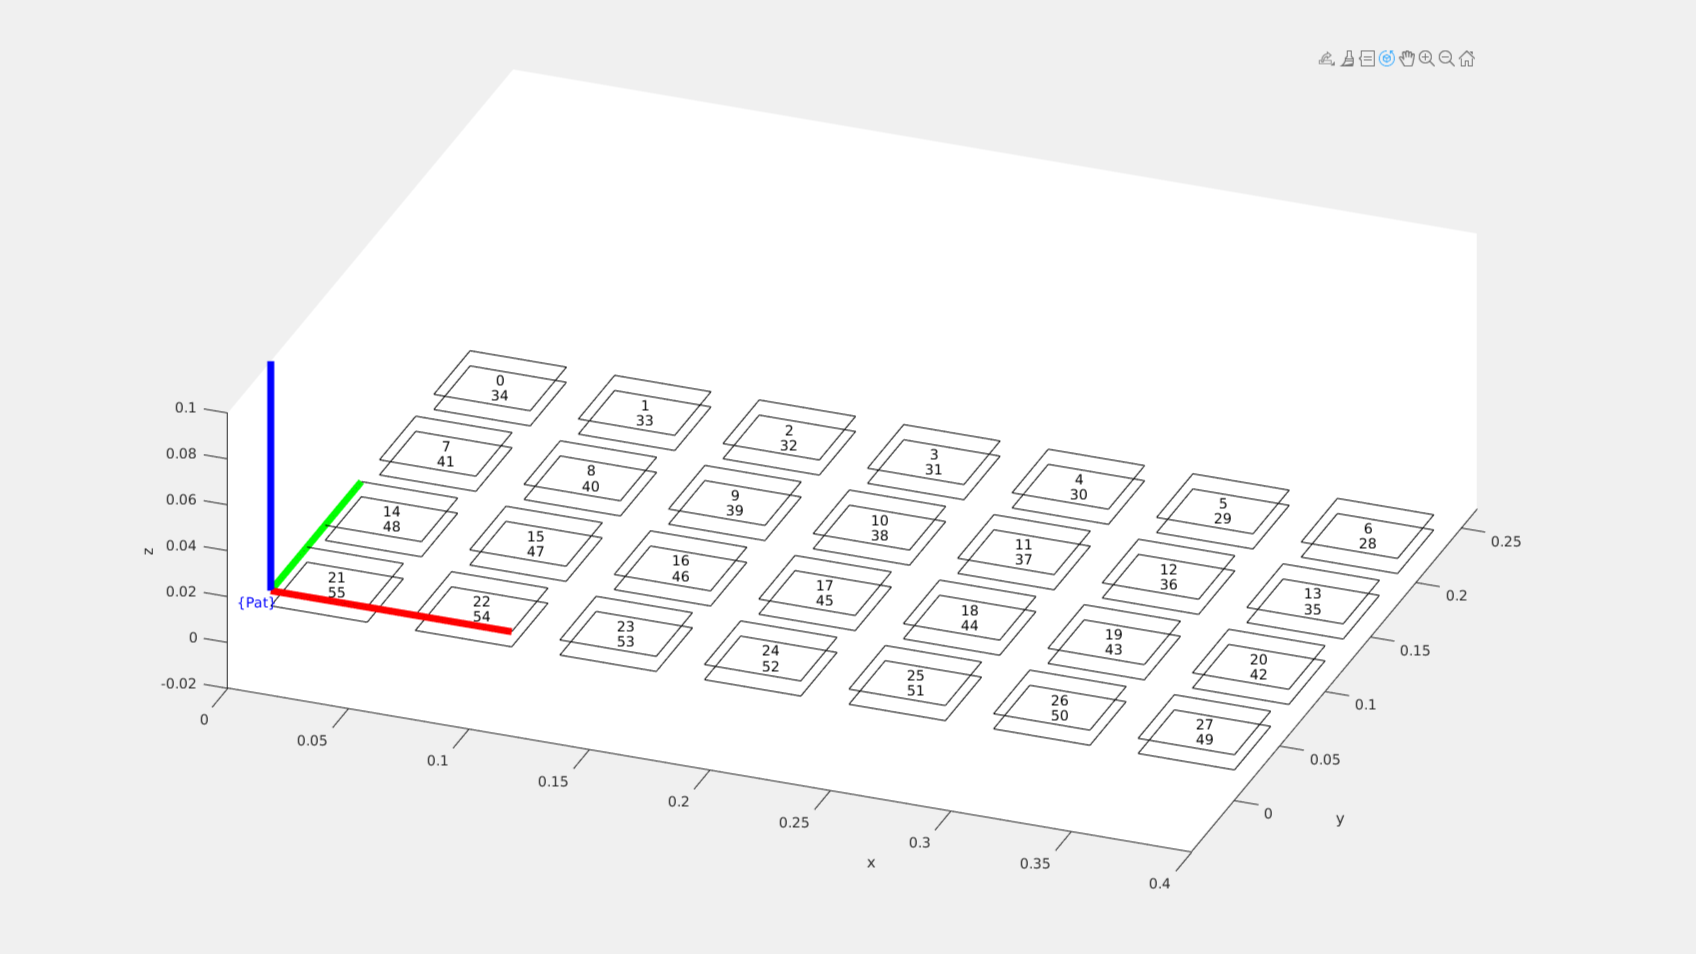
\includegraphics[width=1\textwidth]{Images/ArUco board configuration.png}
\caption{ArUco double-sided board configuration}
\end{figure}

\clearpage
\section{Pose Graph Optimisation}

We propose creating a pose graph, as shown in Figure \ref{fig:posegraph}. The pose graph consists of nodes that are connected by edges, which determines the relative pose between any two corresponding nodes in the graph and can contain uncertainty information of the measurement. The white nodes $X_{k}, k \in \{1,2,..., M\}$ denote the cameras in our system, and the grey nodes $L_{i}, i \in \{1,2,..., N\}$ represent the double-sided ArUco board's origin poses that are detected by at least two cameras. Note that the board pose does not need to be detected by all cameras. Therefore, in the graph each board pose node (grey) must be connected with at least two camera nodes (white), with the edges being the relative poses between the board's origin and the corresponding camera.


\begin{figure}[ht]
\centering
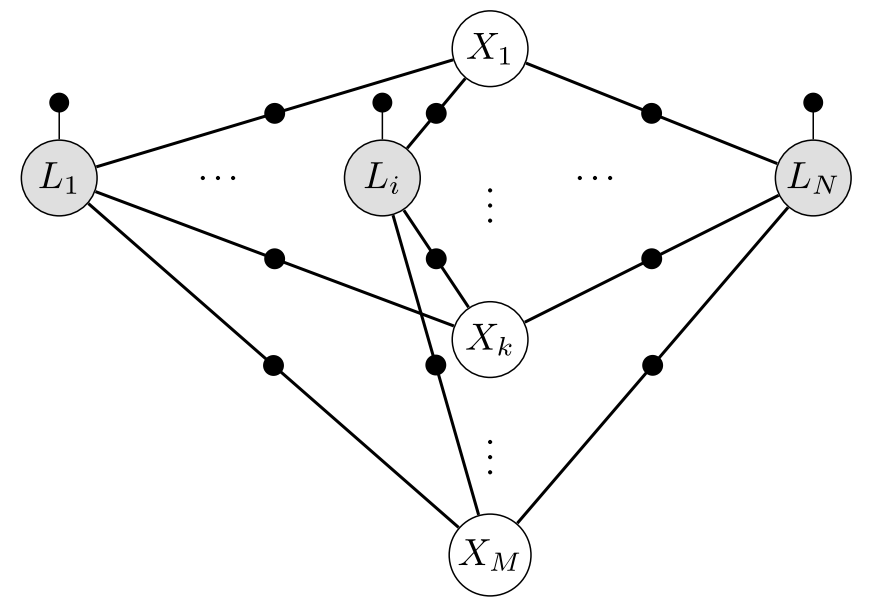
\includegraphics[width=1\textwidth]{Images/pose graph.png}
\caption{Pose Graph represents the calibration method}
\label{fig:posegraph}
\end{figure}